\section{Overview}

The auditory scene presents a complex organizational problem. The sounds in an environment all propagate through the air, and in that medium they mix and mingle. The collection of deviations of air pressure from, say, the sizzling of a steak on a grill, along with those from the laughter of a child, all travel through the same air, and the sum of all these signals is what reaches the ear drum. The hearing apparatus is incredibly sensitive. In perfect silence, humans are sensitive to mechanical vibrations on the eardrum with an amplitude smaller than the deviation of a hydrogen atom. The neurons transcribing the signals from the cochlea have incredible temporal fidelity, faithfully replicating the timing of sound components down to the microsecond. However, these only describe the properties of a one dimensional signal. How does the brain take this exquisitely detailed, but jumbled, information, and decompose it into meaningful information about the environment?

In classical psychology, this is referred to as the "cocktail party problem." In a noisy environment, humans are able to decompose the components of the acoustic signal belonging to different sources, and to group the signal components belonging to the same source together, in order to be able to distinguish one source from another and typically, to focus on a particular sound source or set of sound sources in the environment. For many environments, grouping the frequency components that emanate from the same source can be relatively straightforward. A flute is in a very different frequency range from a tuba, and the various frequencies that are produced by a flute are all similar to each other in time varying modulations (i.e., amplitude or frequency modulation / vibrato), and very different from those of a tuba. However, a number of biologically relevant auditory signals are very similar to each other physically-- predominantly speech.

We aim in the present chapter to review the historical and recent literature regarding this phenomenon, and apply new computational frameworks to existing experimental paradigms, marrying both behavioral and neurobiological evidence.

\section{Background}

\subsection{History of auditory scene analysis}

Building off of the work of Gestalt psychologists in studying visual grouping cues, early researchers tried to understand how sounds were grouped based on similarities, i.e., identical onset times of different frequency components. The idea of competitive grouping emerges \cite{Bregman} as a strategy for understanding auditory perception. Sound components are given "perceptual distance" from one another based on several dimensions, including frequency range, frequency range, timbre, spatial direction, harmonic relationships, comodulations, and fundamental frequency. These relationships describe phenomena observed in both musical composition and speech perception, such as polyphonic composition with a single voice, or the ability to hear a speaker against background noise. Bregman described auditory grouping as stream segregation, with the preprocessing enabling organization of incoming auditory signals into perceptually distinct streams based on psychological similarity being a crucial factor in auditory perception. For instance, it is much easier to compare the relative timing of events within the same auditory stream than those from different putative sources. Through \emph{sequential grouping}, the auditory system is able to link separate auditory events across time, categorizing incoming auditory events into one stream or another by, putatively, the similarity of the sound components, particularly after being mapped from the sound domain into neural representations.

\subsection{Psychological findings}
This premise introduces the possibility for obtaining behaviorally based estimates of a psychological quantity, which should reflect the representation of the stimulus in the nervous system. A typical laboratory experiment of sequential auditory grouping will consist of repeating presentations of some sound A, along with another sound B that is identical to A except for variation some stimulus dimension, such as tone frequency. Through such an approach, psychologists have been able to systematically specify the effect on grouping of frequency difference, as well as perceived location, timbre, pitch, etc. Along with stimulus characteristics ("bottom up", originating in the peripheral nervous system), internal psychological factors of the listener can influence grouping ("top down", originating in the central nervous system)- for instance, if incoming tones comprise a familiar melody, listeners may be inclined to group them, where they may not have been able to form a distinct stream representing the melody without the contribution from stored memories. One factor which probably resides between bottom up and top down processes influencing grouping is the effect of cumulative presentation time - the tendency for stream segregation to "build up" over longer presentations, so that the probability of hearing multiple streams increases with longer exposure times to the stimulus \cite{Bregman1978}, \cite{Anstis1985}, although this can be disrupted by a switch in attention \cite{Cusack2004}.

One of the best studied paradigms for manipulating stream segregation cues is the van Noorden \cite{Noorden1975} experiment \ref{fig:percepts_timecourse}. The stimulus consists of repeating triplets of tones at two different frequencies, A and B, in an ABA\_ pattern. The difference in frequency between tones ($\delta f$) as well as the presentation rate, or tone repetition rate (TRT). At low $\delta f$ or TRT, subjects report hearing the stimulus as grouped, with a galloping rhythm. As the $\delta f$ or the TRT are increased, subjects report hearing the tones split into two different streams with different tempos, one with the A tones and one with the B tones. Often thought of as analogous to figure / ground segregation.

\begin{figure}
	\centering
	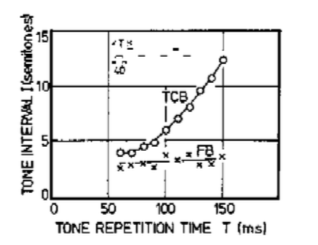
\includegraphics[scale=1.0]{Noorden_Diagram.png}
	\caption{Perceptual states arising under different stimulus parameters for the van Noorden stimulus. Subjects listened to repeating patterns of ABA\_ tones and adjusted a dial to change either the tone repetition rate at which the stimulus was presented, or the difference in frequency, $\delta f$, between the A and the B tones.}
	\label{fig:Noorden_Diagram}
\end{figure}

Interestingly, this stimulus paradigm produces a large range of parameters under which subjects report ambiguity, and undergo alternations between grouped and split percept \cite{Pressnitzer2008}. Therefore, without any change to the stimulus, human subjects can have two completely distinct auditory percepts - allowing us to dissociate the neural underpinnings of some of the more complex processes that underlie auditory perception from basic signal transduction. (NCC?)

Snyder et al, 2009; Cusack et al 2004; van Noorden, 1975; Hupe et al, 2008
Pressnitzer and Hupe asked whether the van Noorden stimulus was a bistable percept \cite{Pressnitzer2005} by modifying the original paradigm and presenting the same stimulus uninterrupted for 4 minutes. During this time, the subjects would continuously report their perceptual state by holding down one button for the "grouped" percept (what they would hear all the time if they were below the "fission boundary" of \ref{fig:Noorden_Diagram}) and another button for the "split" percept (which would be obligatory above the "temporal coherence boundary"), and after a a number of experiments testing research studies since then have , \cite{Pressnitzer2011a}

\subsection{Lessons from visual bistability}

Neuroscientists have a long history of exploiting perceptual illusions to gain information about the nervous system and the signal processing pathways that produce our perceptual experiences. Afterimages reveal color opponency architecture in the retina. Helmholtz. Heeger's V1 imaging, Movshon's plaids, somebody got monkeys to report their percepts. Logothetis? 

Levelt - suggested that rivalry arose from low level processes; did he use mathematical models to support his assertions?

Firing rate vs temporal fine structure

The goal of perception is to tell us about objects in the world, not patterns of excitation at the sense receptors. \cite{Pressnitzer2011a}

Blake and Logothetis \cite{Blake2002} point out that in binocular rivalry, switches are inevitable - whereas in dichotic listening, listeners can stay focused on a particular ear without interruption. Although there are also dichoptic fusions when the images presented to each eye are coherent with each other. It's really a matter of how the particular sensory modality and all its networking has adapted to try to make the most sense out of the types of signals it has coming in - how to guess what's in the outside world.

During rivalry between the eyes, the suppressed percept is accompanied by suppression of those visual inputs in general.
Suppresses excitatory inputs but has no effect on, for instance, adaptation \cite{Blake2002}. Studies using VEPs have shown both spatial segregation of electrical signals from the scalp during different reported dominance phases during binocular rivalry, but also enhanced synchronization in signals from different brain areas during dominance phases, suggesting distributed processing for even a bistable perception paradigm carried through signal differences arising within peripheral channels, i. e., the eyes.


In the case of binocular rivalry, we have the benefit of knowing a lot about the anatomical and functional properties of the brain circuits that underlie each percept - ocular dominance columns provide a distinct anatomical locus. Even with more complex rivalry as with drifting grating / plaids, we know the functional properties of the cells in MT, and they are distinct populations of neurons. With auditory scene alternations, it may be more complicated- the same neurons may be involved with each percept, but with different organizing dynamics (as in dynamical waves/ oscillations). Discrete feature detecting neurons vs dynamic assemblies.



Some other differences with visual signals include occlusion, greater dynamic range and fidelity, much less spatial 


shamma 2008 - Humans are great at separating signal from noise, but we don’t understand the computational principles that allow them to do this. so it’s no wonder we are poor at building engineering systems that can reliably separate an auditory signal from noise.

In particular, our auditory systems remain incredibly flexible - with conscious effort, we can reorganize the incoming pattern of excitation so that different parts of the signal become available to awareness, as when one stops listening to their companion to try to hear someone calling for help. Such capability would be impossible without competition between different representations of the auditory signal according to different groupings. The auditory system seems to represent information at a relatively high level of complexity even without the sensory benefit of attention.

While low level cues are the most straightforward to investigate and model computationally, it should be noted that auditory grouping can be determined by higher order stimulus features, such as statistical regularity (Shamma 2008/ Gutschalk). Systematic study shows perceptual bistability for the van Noorden paradigm, which allows very strong control in the laboratory over the strength of the auditory grouping cues by varying delta f and presentation rate. For most (but not all) listeners, there exists an ambiguous range where listeners report alternating between grouped and split percepts. Alternations have also been observed for higher order stimuli, such as the repeating life / fly ambiguity ("verbal transformations"), suggesting that competition between organizations of sound is a phenomenon that interacts with higher level perceptual signals like speech, which integrates incoming auditory information with stored memory of learned language.

Sue Denham- alternations occur regardless of stimulus parameters if presentations are long enough.

Rivalry between organizations in auditory streaming provides an invaluable opportunity to distinguish between the low level neuronal mechanisms that support the encoding of stimulus features from the specific processes that dictate our perceptions of sound, and the cascade of transformations in between the cochlea and the higher cortices. However, our attempts to isolate the brain activity that form the present percept from that which encodes the stimulus is complicated by the densely recurrent anatomy of the auditory system.

the overall layout should be:
(maybe start with a teaser with some current research that involves stream segregation, i.e. cochlear implants, speech recognition?

psychological findings
streaming
buildup
bistability

anatomy

neural correlates

computational modeling

\subsection{Functional anatomy of the auditory system supporting stream segregation and grouping cues}

\subsubsection{Ascending / afferent pathway}
The process of turning the one dimensional signal transmitted through the ear drum into complex representations of distinct auditory objects begins in the cochlea, the snail shaped organ in the inner ear. After the mechanical vibrations of the ear drum, amplified by the malleus, incus, and stapes of the middle ear, are transferred through the oval window into the watery liquid of the perilymph, the cochlea is able to exploit the fluid dynamics and elasticity along the basilar membrane to spatially segregate the one dimensional signal from the ear drum by frequency components. High energy treble produces strong vibrations on the stiff base of the basilar membrane, while the thinner apex of the cochlea responds to bass components. Depending on the treble or bass in the sound wave, different regions of the membrane will be deformed, pulling open the tip links on the end of long, slender stereocilia, hair cells embedded in the epithelium of the basilar membrane called the organ of Corti, allowing ions to rush in and the depolarizations that cause the neurites to change their release of neurotransmitter. To boost the signal even further, the outer hair cells - which outnumber the inner hair cells 4 to 1 - provide electromotile amplification, as well as gain control, of the motion of the basilar membrane. The physical separation in space of the waveform by these mechanical events roughly reproduces the Fourier transform, mapping a time-varying signals into a frequency spectrum. However, the question of which parts of the sound signal belong to which sources in the environment is still unsolved.

After the spatial segregation of the sound wave into its spectral components along the basilar membrane, the auditory system tends to maintain a roughly tonotopic map, where neurons that are close together tend to respond to stimulation from similar sound frequencies. The passive potentials of the inner hair cells of the cochlea release glutamate onto the dendrites of the spiral ganglion, an exquisite feature containing dense innervation with ribbon synapses from the base of the hair cells, which enables high temporal fidelity encoding the precise timing of auditory signals from lower frequencies. The axons of these neurons forming the auditory nerve, along with those from the vestibular system, project ipsilaterally through the cranial nerve VIII to the cochlear nucleus (CN) in the brainstem. Here, different excitatory cell types are selective for different aspects of the stimulus - some are more sensitive to timing, some have high frequency selectivity, some have intrinsic rhythm selectivity, and some are level-dependent. In particular, type IV or fusiform cells of the dorsal cochlear nucleus integrate multiple frequencies to create spectral selectivity that provides elevation information for sound localization. The selectivity of cells in the CN seems to dramatically depend on the activity of inhibitory interneurons \cite{evans2013} and can be strongly disrupted by anesthesia, affecting all subsequent processing of auditory afferents. The CN is therefore more than just a relay, and the afferents leaving its nuclei are imparted with more information than was available in the auditory nerve. 

These variously project to different areas of the brain stem; the medial nucleus of the the trapezoid body (MNTB) of the superior olivary complex receives the first crossed signals, where information from the two ears converge. The enables the extraction of spatial localization information; the lateral superior olive (LSO) extracts information from the microsecond-magnitude differences in timing as sound sources reach one ear before the other (interaural time differences, or ITD), whereas the medial superior olive (MSO) compares the level differences between the two ears (interaural level differences, ILD). Spatial cues can assist in segregation of sounds in different locations, but these cues are not determinative of sound source- in fact, sounds presented separately to each ear can be fused into a singular complex percept, as in sine wave speech \cite{Remez1994}, in which sine-wave replications of the formants of a speech utterance, even when presented dichotically, are possible to fuse to perceive and extract linguistic information. Sound echoes in natural environments make spatial cues somewhat unreliable in determining the grouping of sound components belonging to a single source. Another target of projections from the CN is the lateral lemniscus, a superhighway of auditory nerve fibers that carries auditory afferents throughout the brainstem while also introducing some GABAergic inhibition. The neurons within have distinct types encompassing both phasic responses to sound onsets as well as tonic responses with sustained firing for the duration of the sound.

The lateral lemniscus carries nerve signals from CN and LSO to the inferior colliculus (IC) of the midbrain, where cells with more complex stimulus selectivity begin to emerge. The central nucleus of the IC is an integration center for the vast majority of auditory afferent pathways, organized tonotopically into frequency-band selective laminae. A mix of monaural, binaural, monosynaptic, or multisynaptic information from the ears are available, providing a rich array of different calculations extracted from the auditory signal from the ears, with both excitatory and inhibitory interactions. IC also receives inputs from visual system subserving orienting and startle responses. Here vertical and horizontal orientation information converge, and amplitude-modulation (AM) selective cells emerge - cells that are tuned for (or against) a particular modulation frequency, as well as phase locking with the envelope of the modulation frequency \cite{Rabang2012}. In addition, there are excitatory and inhibitory connections between the left and right inferior colliculi, further enabling integration of information from previous processing stages. These different groups of cells with different response properties project to the ventral aspect of the medial geniculate body (MGB) of the thalamus along fine tuned topographic relays, primarily carrying binaural information. There are populations of frequency, intensity, location, and modulation selective cells within the various sub-nuclei of the MGB, along with intrathalamic interneurons projecting onto both excitatory and inhibitory (i.e., disinhibition) circuits. 

These cells project to primary auditory cortex (A1), located bilaterally in the Sylvian fissure including the superior temporal gyrus in humans, along with several auditory association areas. Lesions to A1 produce cortical deafness, indicating that cortical processing is required for auditory awareness, although auditory reflexes can remain intact. Some neurons in A1 display selectivity for pitch, as well as harmonicity, suggesting information of information from multiple frequency bands from the thalamic inputs. In addition to the primary auditory cortex ("core"), 

From there it goes to the cochlear nucleus, and from there it goes to the inferior colliculus. From there it goes to the auditory cortex, and there's a lot of auditory association cortex nearby. 

primary auditory cortex and its belt
Because of the architecture of the auditory system, there is an exquisite potential for attention or other top down processes (i.e., familiarity) to influence the low level cues, even the encoding of the stimulus. Descending projections from AC can modulate neural responses all along the outer hair cells in the cochlea, changing its localized stiffness and therefore changing the sensitivity of the sensory transducer to different frequency bands\cite{Terreros2015}. This makes the quest for neural correlates of auditory object formation complicated, as does the fact that most auditory cortex neurons exhibit different response properties under anesthesia.

Binding could likely recruit some mechanisms outside of auditory cortex, as in the intraparietal sulcus; \cite{Carlyon2001}
\subsection{Neurobiological findings so far}
Micheyl et al, Bee, etc, Fishman, 

SSA

MMN

Auditory attention seems to involve a very strong inhibitory component


\subsection{Computational methods for investigating perception}

Although large scale neuronal recording techniques have evolved rapidly over the last several years, there are not only ethical but logistical constraints in recording from neurons during higher order perceptual judgments and processes - although there have been some ECG studies in recent years. But even advances in measuring brain responses don't eliminate the difficulty in recording from all of the cells involved.

Computational methods are less invasive. There's a lot of success in using computational methods to provide a framework for understanding neurobiological properties, as well as to generate predictions and constrain future biological studies. In particular, methods from visual binocular rivalry and other bistable perception has been helpful for understanding mechanisms of visual perception 

Wilson Cowan model



\section{Present investigation}

How much of the brain activity can be attributed to the encoding of the stimulus attributes, and how can that be distinguished from the brain activity that specifically organizes those encoded signals into our perceptions of sound sources? Perceptual bistability provides an invaluable test bed, because the underlying physical signals remain unchanged while the perceptions change. 
\section{The stimulus}

We use repeating triplets at two frequencies A and B, separated by a silent interval \_ (ABA\_). Depending on the difference in frequency of the tones ($\Delta f$), as well as the presentation rate ($PR$), the subject may perceive the sound stimulus as either a single source with a galloping rhythm, or as two simultaneous sounds. See \ref{fig:percepts_timecourse} 

\subsection{The task}

Subjects hold one of two buttons to indicate whether they hear the grouped percept with a galloping rhythm or a split percept in which each of the two tone frequencies appear to be segregated in distinct streams with isochronous rhythms. 


\begin{figure}
	\centering
	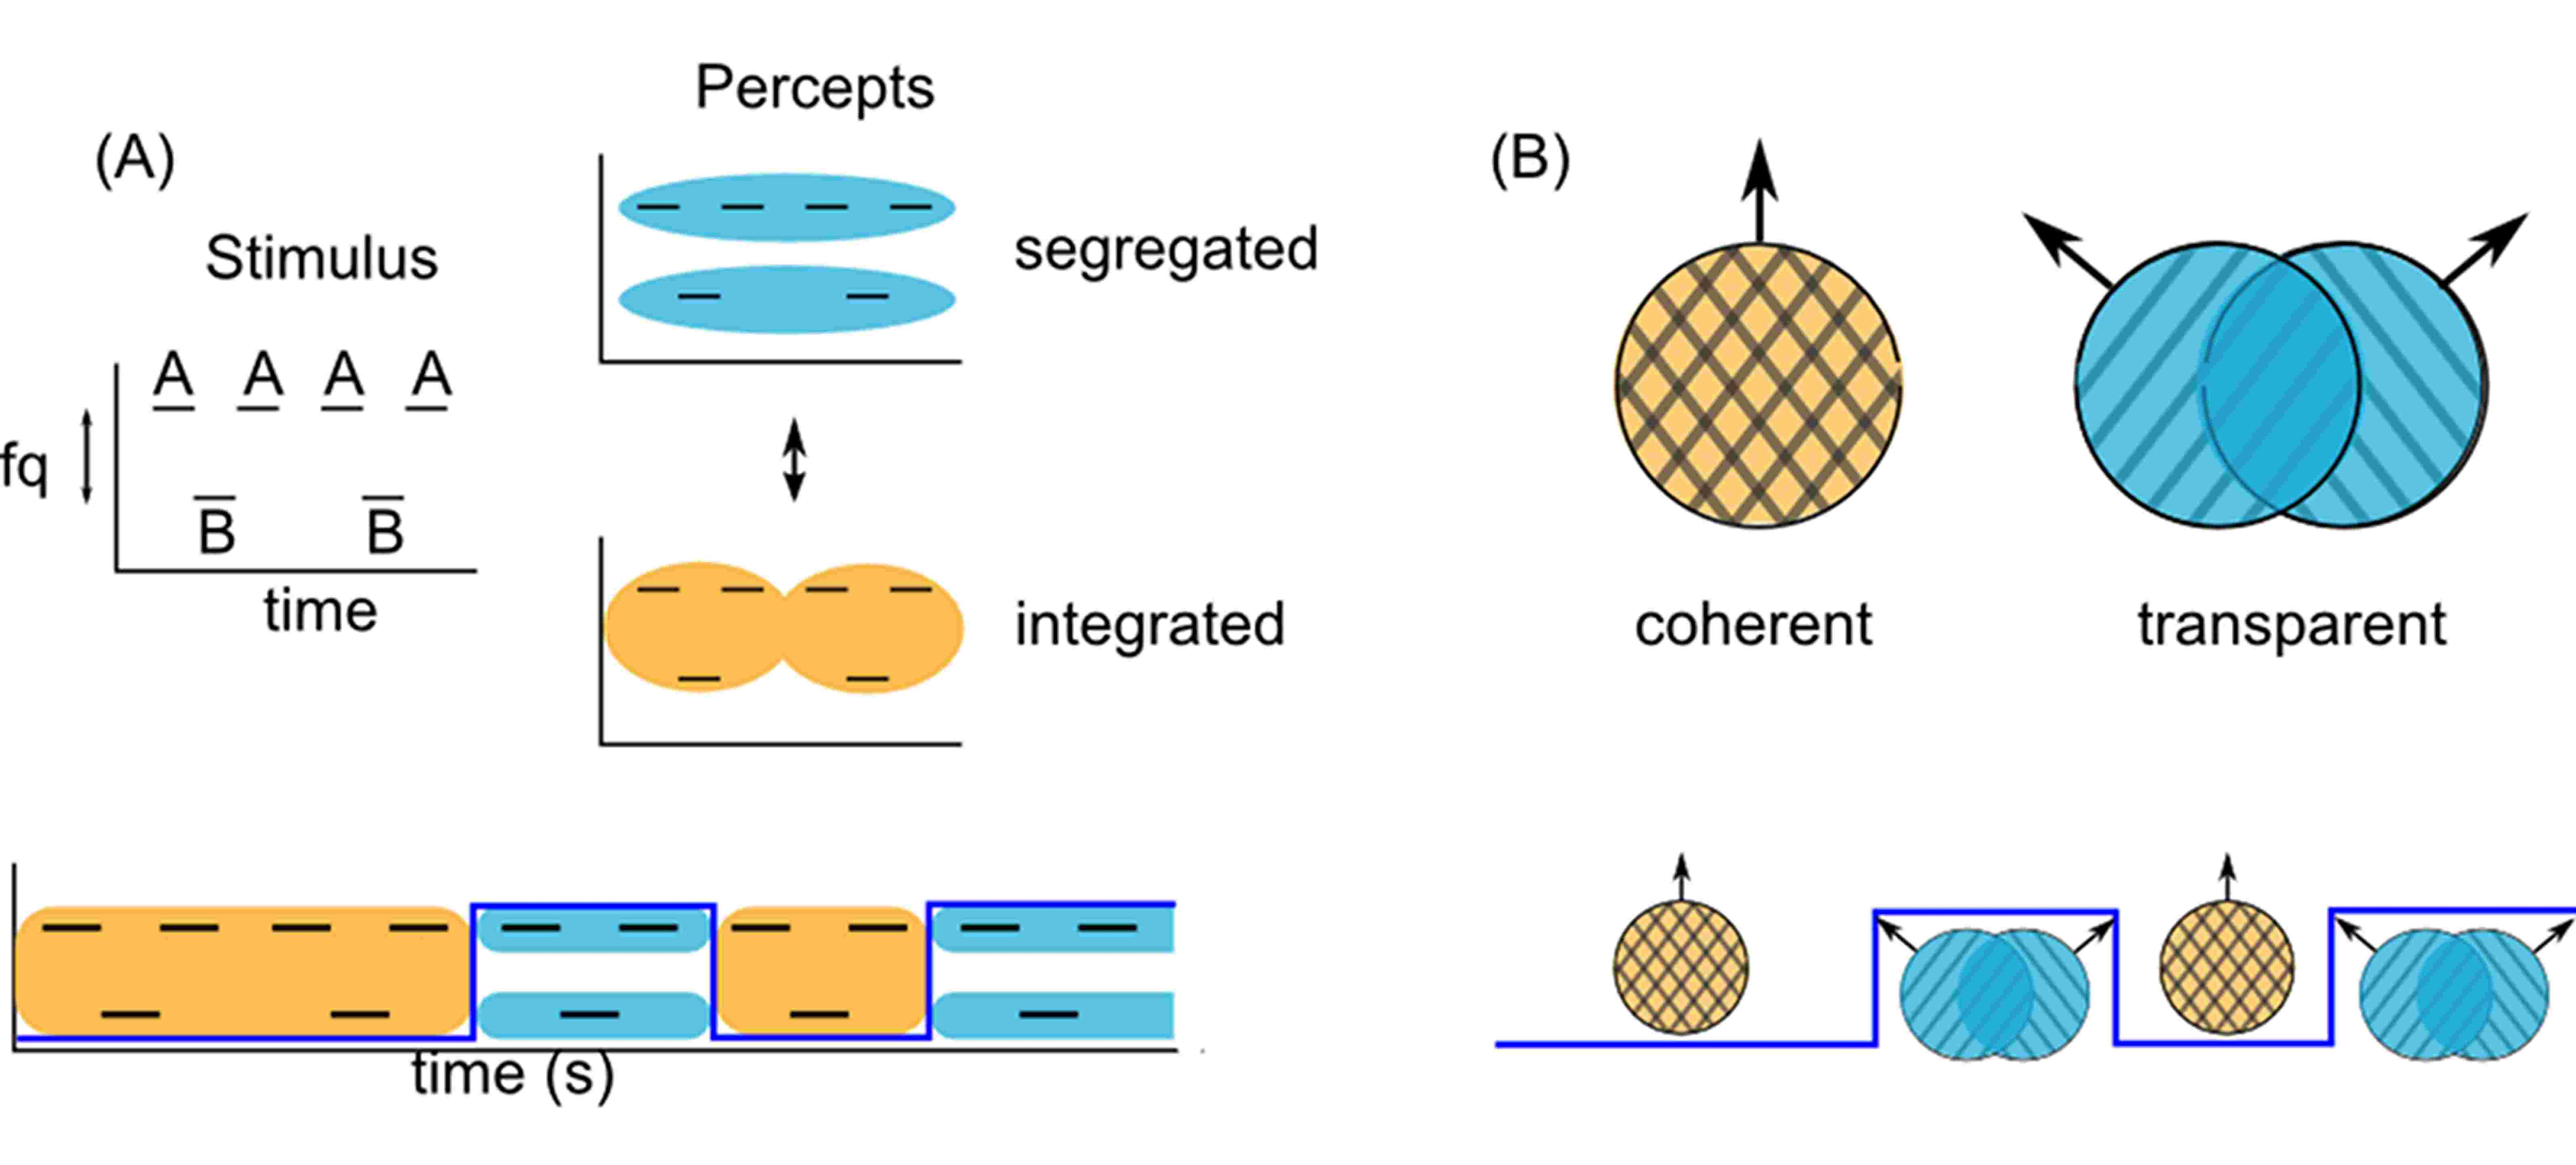
\includegraphics[scale=0.7]{1-aba_stim_percepts.jpg}
	\caption{Examples of stimuli that can produce ambiguous grouping. \textbf{(a)} Van Noorden triplets with ambiguous stream segregation. Listeners report alternations between hearing integration (bottom, orange) and segregation (top, blue) of the component tone frequencies. \textbf{(b)} Moving gratings at certain angles can produce ambiguous motion. Observers report alternations between coherent and transparent motion of the component gratings.}
	\label{fig:percepts_timecourse}
\end{figure}



